% Este é o arquivo principal, onde o seu trabalho é gerado
% Se tiver dúvidas, leia os comentários ou as referências
% da biblioteca ABNTeX 2.
% Ou também consulte http://aureliocasoni.xyz/latex
\documentclass[12pt,oneside,chapter=TITLE,
    section=TITLE,a4paper,english,brazil,sumario=abnt-6027-2012,]{abntex2}
\tracingoutput
\tracingmacros

% Remove as advertências bizarras de inclusão de pacotes em subpastas. 
\usepackage{silence}
%Disable all warnings issued by latex starting with "You have..."
\WarningFilter{latex}{You have requested package}

\usepackage{include/unigran}

\usepackage[T1]{fontenc}		% Selecao de codigos de fonte.
\usepackage{lastpage}			% Usado pela Ficha catalográfica
\usepackage{indentfirst}		% Indenta o primeiro parágrafo de cada seção.
\usepackage{color}				% Controle das cores

\usepackage{adjustbox}

\usepackage{longtable,ltcaption} % para as tabelas

\usepackage{amssymb}
\usepackage{amsmath}
\usepackage{amsthm}


\usepackage{helvet}			% Usa a fonte Latin Modern			
%\usepackage{lmodern}			% Usa a fonte Latin Modern			
\usepackage[utf8]{inputenc}		% Codificacao do documento (conversão automática dos acentos)
			% Controle das cores
\usepackage{graphicx}			% Inclusão de gráficos
\usepackage{caption}
\usepackage{subcaption}
%\usepackage{subfig}
%\captionsetup[subfigure]{labelfont=rm}
\newcommand{\subfigref}[1]{\hyperref[#1]{Figura~\ref*{#1}}}
\usepackage{float}
\usepackage{url}
\usepackage{multirow}
\usepackage{textcomp}
\usepackage{microtype} 			% para melhorias de justificação
\usepackage{enumerate}
\usepackage{enumitem}
\usepackage{amsmath}
\usepackage{siunitx}

\usepackage{varwidth}
\usepackage{multirow} % Mesclar linhas
\usepackage{microtype} 			% para melhorias de justificação

\usepackage{pdfpages}  
\usepackage{tocloft}                                % Permite alterar a formatação do Sumário
\usepackage{etoolbox}                               % Usado para alterar a fonte da Section no Sumário

\usepackage{lipsum}
% ---
% Pacotes de citações
% ---
%\usepackage[brazilian,hyperpageref]{backref}	 % Paginas com as citações na bibl
\usepackage[alf, abnt-etal-text=emph, abnt-dont-use-etal=yes, bibjustif]{abntex2cite}	         % Citações padrão ABNT

\usepackage{include/url6023} % remove os <> entre a Url, segundo a nova versão da NBR 6023:2018
% se, em uma futura atualização completa do Abntex, isso causar erros na geração da Url, pode comentar na linha acima
% https://github.com/abntex/abntex2/issues/210


% ---

% --- 
% CONFIGURAÇÕES DE PACOTES
% --- 

% ---
% Configurações do pacote backref
% Usado sem a opção hyperpageref de backref
%\renewcommand{\backrefpagesname}{Citado na(s) página(s):~}
% Texto padrão antes do número das páginas
%\renewcommand{\backref}{}
% Define os textos da citação
% \renewcommand*{\backrefalt}[4]{
% 	\ifcase #1 %
%		Nenhuma citação no texto.%
%	\or
%		Citado na página #2.%
%	\else
%		Citado #1 vezes nas páginas #2.%
%	\fi}%
% ---
%configuração para a lista de quadros
%%% nome para ser usado no sumário

%%%%%%%%%%%%%%%%%%%%%%%%%%%%%%%%%%%%
%Informação para configuração das figuras
\newcommand{\source}[1]{\caption*{Fonte: {#1}} }
% ---
% Informações de dados para CAPA e FOLHA DE ROSTO
% Preencha com bastante atenção!
% ---
% Título do seu trabalho
\titulo{Título da tese ou dissertação}

% Nome(s) do(s) autor(es) do seu trabalho. Se tiver mais de um, separe-os com \\
% Se não for uma monografia, coloque o seu RGM
\autor{Nome do candidato}

% Exemplo de dois autores - Ponha um \\ entre eles e remova os %
% \autor{JOSÉ CARLOS ALVES RGM - 99.603\\
% FULANO - RGM xx.XXX}

% Local, nem precisa mexer
\local{Duque de Caxias - RJ}

% Ano do seu trabalho
\data{20aa}

%\renewcommand{\orientadorname}{Orientadora:} %caso seja mulher, apague o % no início da linha

% Nome do seu orientador
\orientador{Nome do Orientador(a)}

%\renewcommand{\coorientadorname}{Coorientadora:} %caso seja mulher
% Coorientador, se não tiver, coloque um % antes dessa linha
\coorientador{Nome do Coorientador(a)}
 
\tipotrabalho{[Dissertação de Mestrado][Tese de doutorado][Monografia para Qualificação ao Doutorado]}
% Se não for monografia, coloque Pré-Projeto, Relatório, Trabalho, etc

% O preambulo deve conter o tipo do trabalho, o objetivo, 
% o nome da instituição e a área de concentração 
\preambulo{\imprimirtipotrabalho apresentada ao Programa de Pós-Graduação em [Biotecnologia] [Metrologia] [Metrologia e Qualidade] do Instituto Nacional de Metrologia, Qualidade e Tecnologia como parte dos requisitos para a obtenção do título de [Mestre] [Doutor] em Ciências.}
% ---

\def \b{$\bullet$}


% ----
% Início do documento
% ----
\begin{document} %Não remova esta linha!

% Retira espaço extra obsoleto entre as frases.
\frenchspacing 

% ----------------------------------------------------------
% ELEMENTOS PRÉ-TEXTUAIS
% ----------------------------------------------------------
\pretextual

\pagenumbering{roman}

% ---
% Capa
% ---
\imprimircapa
% ---

% ---
% Folha de rosto
% (se você digitar \imprimirfolhaderosto* indica que haverá a ficha bibliográfica)
% Mas como a ficha é feita depois, não precisa colocar
% ---
\imprimirfolhaderosto
% ---

% Isto é um exemplo de Ficha Catalográfica, ou ``Dados internacionais de
% catalogação-na-publicação''. Você pode utilizar este modelo como referência. 
% Porém, provavelmente a biblioteca da sua universidade lhe fornecerá um PDF
% com a ficha catalográfica definitiva após a defesa do trabalho. Quando estiver
% com o documento, salve-o como PDF no diretório do seu projeto e substitua todo
% o conteúdo de implementação deste arquivo pelo comando abaixo:
%
% \begin{fichacatalografica}
%     \includepdf{fig_ficha_catalografica.pdf}
% \end{fichacatalografica}
\begin{fichacatalografica}
	\centering Catalogação elaborada pela Biblioteca do Inmetro
	
	
		\noindent\fbox{\begin{minipage}{\dimexpr\textwidth-2\fboxsep-2\fboxrule\relax}


	\imprimirautor
	
	\hspace{0.5cm} \imprimirtitulo  / \imprimirautor. --
	\imprimirlocal, \imprimirdata-
	
	\hspace{0.5cm} \pageref{LastPage} p. : il. (algumas color.) ; 30 cm.\\
	
	\hspace{0.5cm} \imprimirorientadorRotulo~\imprimirorientador\\
	
	\hspace{0.5cm}
	\parbox[t]{\textwidth}{\imprimirtipotrabalho~--~\imprimirinstituicao,
	\imprimirdata.}\\
	
	\hspace{0.5cm}
		1. Palavra-chave1.
		2. Palavra-chave2.
		I. Orientador.
		II. Universidade xxx.
		III. Faculdade de xxx.
		IV. Título\\ 			
	
	\hspace{8.75cm} CDU 02:141:005.7\\
	
	\end{minipage}}

	
	
\vspace*{\fill}	
\vspace*{\fill}	

\begin{flushleft}
{\bfseries REFERÊNCIA BIBLIOGRÁFICA}

SOBRENOME, Nome do autor. \imprimirtitulo. \imprimirdata. nnf. \imprimirtipotrabalho em Metrologia – \imprimirinstituicao, \imprimirlocal, \imprimirdata.
	
\vspace*{\fill}		
	
{\bfseries CESSÃO DE DIREITOS}

NOME DO AUTOR: \imprimirautor.

TÍTULO DA MONOGRAFIA: \imprimirtitulo.

TIPO DE MONOGRAFIA: \imprimirtipotrabalho em Metrologia / \imprimirdata.


É concedida ao Instituto Nacional de Metrologia, Qualidade e Tecnologia a permissão para reproduzir e emprestar cópias desta monografia somente para propósitos acadêmicos e científicos. O autor reserva outros direitos de publicação.
\vspace*{\fill}	

	\rule[-2cm]{3in}{0.1pt}
	
	\imprimirautor\\
	Endereço completo do autor, Bairro, Cidade, UF - CEP xx.xxx-xxx.
	
	\end{flushleft}
\end{fichacatalografica}
% Isto é um exemplo de Folha de aprovação, elemento obrigatório da NBR
% 14724/2011 (seção 4.2.1.3). Você pode utilizar este modelo até a aprovação
% do trabalho. Após isso, substitua todo o conteúdo deste arquivo por uma
% imagem da página assinada pela banca com o comando abaixo:
%
% \includepdf{folhadeaprovacao_final.pdf}
%
% ESQUEÇA ISSO, O CURSO FORNECERÁ UMA ASSINADA.
% ASSIM, NEM SE PREOCUPE COM ISSO.
%
\begin{folhadeaprovacao}

 \begin{center}
    {\ABNTEXchapterfont\large\imprimirautor}

    \vspace*{\fill}\vspace*{\fill}
    \begin{center}
      \ABNTEXchapterfont\bfseries\Large\imprimirtitulo
    \end{center}
    \vspace*{\fill}
    
    \hspace{.45\textwidth}
    \begin{minipage}{.5\textwidth}
       A presente [Dissertação] [Tese] [Monografia de Qualificação para o Doutorado], apresentada ao Programa de Pós-Graduação em [Biotecnologia] [Metrologia] [Metrologia e Qualidade] do Instituto Nacional de Metrologia, Qualidade e Tecnologia como parte dos requisitos para a obtenção do título de [Mestre] [Doutor]em Ciências, foi aprovada pela seguinte Banca Examinadora:
    \end{minipage}%
    \vspace*{\fill}
   \end{center}
        
   %Trabalho aprovado. \imprimirlocal, 30 de maio de 2022:

   \assinatura{Doutor(a) {\imprimirorientador \:- Inmetro} \\ Presidente da banca examinadora} 
   \assinatura{Doutor(a) {\imprimircoorientador \:- Inmetro} \\ }
   \assinatura{{Doutor(a) Nome do avaliador 1 (Interno ao PPG) - Filiação} \\ }
   \assinatura{{Doutor(a) Nome do avaliador 2 (Externo ao Inmetro) - Filiação} \\ }
   \assinatura{{Doutor(a) Nome do avaliador 3 - Filiação} \\ }
      
   \begin{center}
    \vspace*{0.5cm}
    {\large Duque de Caxias, dd de mês de \imprimirdata}
    \vspace*{1cm}
  \end{center}
  
  
\end{folhadeaprovacao}
% ---

% Errata, só é aplicado caso haja um erro no seu trabalho
%% ---
% Inserir errata
% Use se for necessário, não é obirgatório
% ---
\begin{errata}
%Elemento opcional da NBR14724:2011. Exemplo:

\vspace{\onelineskip}

%nao remova esta linha
\noindent 
%Abaixo, faça uma auto-referência do seu trabalho
FERRIGNO, C. R. A. \textbf{Tratamento de neoplasias ósseas apendiculares com
reimplantação de enxerto ósseo autólogo autoclavado associado ao plasma
rico em plaquetas}: estudo crítico na cirurgia de preservação de membro em
cães. 2011. 128 f. Tese (Livre-Docência) - Faculdade de Medicina Veterinária e
Zootecnia, Universidade de São Paulo, São Paulo, 2011.

\begin{table}[htb]
\center
\footnotesize
\begin{tabular}{|p{1.4cm}|p{1cm}|p{3cm}|p{3cm}|}
  \hline
   \textbf{Folha} & \textbf{Linha}  & \textbf{Onde se lê}  & \textbf{Leia-se}  \\
    \hline
    1 & 10 & auto-conclavo & autoconclavo\\
   \hline
\end{tabular}
\end{table}

\end{errata}
% ---


% Os três itens a seguir, são mais usuais se você estiver redigindo sua monografia.
% ---
% Dedicatória
% Texto vindo do modelo original ABNTeX
% Altere-o livremente
% ---
%DEDICATÓRIA, CONFORME A NORMA NBR14724/2011 NÂO POSSUI TÍTULO
\begin{dedicatoria}
   \vspace*{\fill}
   \centering
   \noindent
   \textit{ A dedicatória é opcional. Caso não seja feita dedicatória, esta página deverá ser excluída. Normalmente a dedicatória aparecerá apenas na versão final do texto enviado para a banca examinadora, sendo desnecessária em etapas intermediárias, como por exemplo os Seminários de Acompanhamento de Projetos (SAP) ou Qualificação para o Doutorado.
A dedicatória é um texto normalmente de foro íntimo, onde pessoas queridas são mencionadas. As referências a colegas, orientadores, docentes, técnicos e pessoal de apoio administrativo costumam ser feitas nos Agradecimentos.
A definição da norma ABNT NBR 14724:2011 é “texto em que o autor presta homenagem ou dedica seu trabalho” (item 3.9).
} \vspace*{\fill}
\end{dedicatoria}
% ---
% ---
% Agradecimentos
% ---
\begin{agradecimentos}
Os agradecimentos são opcionais. Caso haja apoio financeiro para a execução do projeto, principalmente de agências de fomento ou empresas privadas, o apoio deverá ser mencionado nos agradecimentos. Preferencialmente, a critério do orientador, deverão ser incluídos os números de processo dos financiamentos de agências de fomento.

Apoios não financeiros devem ser inseridos nesta seção da monografia. É importante reforçar que “Dedicatória” e “Agradecimentos” têm propósito distintos, portanto não devem ser confundidas suas propostas numa dissertação.

Caso não sejam feitos agradecimentos, esta página deverá ser excluída. Normalmente os agradecimentos aparecerão apenas na versão final do texto enviado para a banca examinadora, sendo desnecessários em etapas intermediárias, como por exemplo os Seminários de Acompanhamento de Projetos (SAP) ou Qualificação para o Doutorado.

A definição da norma ABNT NBR 14724:2011 é “texto em que o autor faz agradecimentos dirigidos àqueles que contribuíram de maneira relevante à elaboração do trabalho” (item 3.2).

\end{agradecimentos}
% ---
% ---
% Epígrafe
% Texto vindo do modelo canônico ABNTeX 2
% Altere-o livremente.
% ---
\begin{epigrafe}
    \vspace*{\fill}
  %EPÍGRAFE, CONFORME A NORMA NBR14724/2011 NÂO POSSUI TÍTULO
  
    %APAGAR ESTA PARTE NO MODELO FINAL:
    %%%%%%%%%%%%%%%%%%%%%%%%%%%%%%%%%%%%%%%%%%%%
Epígrafe é opcional. Caso seja inserida no texto, ela deve ser elaborada conforme a ABNT NBR 10520. Deve ser inserida após os agradecimentos. Podem também constar epígrafes nas folhas ou páginas de abertura das seções primárias, ou seja, ao início de cada capítulo da monografia. O tipo de letra da epígrafe pode ter algum tipo de efeito “artístico”.

Caso não seja feita epígrafe, esta página deverá ser excluída. Normalmente a epígrafe aparecerá apenas na versão final do texto enviado para a banca examinadora, sendo desnecessária em etapas intermediárias, como por exemplo os Seminários de Acompanhamento de Projetos (SAP) ou Qualificação para o Doutorado.

A definição da norma ABNT NBR 14724:2011 é “texto em que o autor apresenta uma citação, seguida de indicação de autoria, relacionada com a matéria tratada no corpo do trabalho” (item 3.14).

Veja um exemplo a seguir:
%%%%%%%%%%%%%%%%%%%%%%%%%%%%%%%%%%%%%%%%%%%%%%%%
	\begin{flushright}
		\textit{`A linguagem, tanto falada quanto escrita, é viva, dinâmica e sofre adaptações ou aperfeiçoamentos ao longo do seu uso. A linguagem técnica, entretanto, é tida como perene, sendo, em muitos casos, claramente rechaçadas tentativas de inserção de novos termos em algumas áreas clássicas. Não se pode afirmar de maneira inconteste que esse conceito seja irrestrito, posto que muitas áreas da ciência dependem e evoluem com as novidades ou inovações tecnológicas. A metrologia, nesse contexto, embora seja uma ciência clássica, vem se desenvolvendo calcando-se em aprimoramentos tecnológicos, o que lhe transfere um dinamismo natural dos termos e conceitos empregados.
(OLIVEIRA; COSTA-FELIX, 2017, p. 45).
}
	\end{flushright}
\end{epigrafe}
% ---

% ---
% RESUMOS
% ---
\setlength{\absparsep}{18pt} % ajusta o espaçamento dos parágrafos do resumo

% Inclui os arquivos de resumo
% Usual apenas para monografia, ou se seu professor exigir
% Se não precisar, apague a(s) linha(s) ou coloque um % antes
\begin{resumo}
    %remova estas linhas e troque pelo seu conteúdo
    O resumo na língua vernácula é um elemento pré-textual obrigatório. O resumo deve ser elaborado conforme a ABNT NBR 6028.O resumo de monografia deve ter entre 150 e 500 palavras em um único parágrafo. O resumo deve conter a contextualização do problema, o “gap” ou lacuna no estado da técnica, a solução proposta ou objetivos do trabalho, a abordagem ou metodologia empregada, os principais resultados, breves discussão e conclusão. Vejam as videoaulas do Professor Zucolotto \cite{Zucolotto} e as notas de aula da disciplina de Metodologia da Pesquisa para exemplos e detalhes de como fazer um bom resumo.
    
    %troque por suas palavras-chave
    \palavraschave{palavra-chave 1, palavra-chave 2, palavra-chave 3}
    %[entre 3 e seis palavras-chave, em ordem alfabética, separadas por ponto e vírgula e finalizadas por ponto; esta formatação diverge da apresentada na norma ABNT NBR 6028]
\end{resumo}
\begin{resumo}[Abstract]
    %\begin{otherlanguage*}[english]
    % You haven't defined the language [ yet.
        %remova esta linha e troque pelo seu conteúdo
        
        The abstract shall be an English version as close to the Portuguese version as possible, following the same structure.
        %troque por suas palavras-chave
        \keywords{palavra-chave 1, palavra-chave 2, palavra-chave 3}
    %\end{otherlanguage*}
\end{resumo}

% ---
% inserir lista de ilustrações
% ---
\pdfbookmark[0]{\listfigurename}{lof}
\listoffigures*
\cleardoublepage
% ---
% inserir lista de quadros
% ---
\pdfbookmark[0]{\listtablename}{lot}
\listofquadros*
\cleardoublepage

% ---
% ---
% inserir lista de tabelas
% ---
\pdfbookmark[0]{\listtablename}{lot}
\listoftables*
\cleardoublepage
% ---

% ---
% insere a lista de algoritmos
% veja o algoritmo de exemplo e as linhas 250 a 275 do arquivo 
% unigran.sty para saber as palavras-chave
% ---
%\imprimirlistadealgoritmos

% ---
% inserir lista de codigos-fonte
% ---
%\imprimirlistadecodigosfonte

% ---
% inserir lista de abreviaturas e siglas
% ---
\chapter*{Lista de Abreviaturas e Siglas}
%%%%%%%%%%%%%%%%%%%%%%%%%%%%%%%%%%%%%%%%%%%%%%%%
%Elemento opcional. Consiste na relação alfabética das abreviaturas e siglas utilizadas no texto, seguidas das palavras ou expressões correspondentes grafadas por extenso. Recomenda-se a elaboração de lista própria para cada tipo, ou seja, uma lista para abreviaturas e outra para siglas.
%Segundo a norma técnica ABNT NBR 14724:2011, abreviatura é a “representação de uma palavra por meio de alguma(s) de sua(s) sílaba(s) ou letra(s)” (item 3.1).
%Segundo a norma técnica ABNT NBR 14724:2011, sigla é o “conjunto de letras iniciais dos vocábulos e/ou números que representa um determinado nome” (item 3.28).
%%%%%%%%%%%%%%%%%%%%%%%%%%%%%%%%%%%%%%%%%%%%%%%%%

\begin{tabular}{lll}
  USB     & & {\em Universal Serial Bus} \\
  CPU     & & {\em Central Processing Unity}\\
  HDMI    & & {\em High Definition Multimedia Interface}\\
  RAM     & & {\em Random Access Memory}\\
\end{tabular}
\clearpage
% ---
% inserir lista de simbolos
% ---
\chapter*{Lista de Símbolos}
%EXCLUIR ESSA PARTE

%%%%%%%%%%%%%%%%%%%%%%%%%%%%%%%%%%%%%%%%%%%%%%%%
%Elemento opcional. Elaborada de acordo com a ordem apresentada no texto, com o devido significado. Os símbolos não são listados por ordem alfabética porque não são siglas ou abreviaturas.
%%%%%%%%%%%%%%%%%%%%%%%%%%%%%%%%%%%%%%%%%%%%%%%%
\begin{tabular}{lll}
  $\Gamma$   & & {\em Letra grega Gama} \\
  $\Lambda$     & & {\em Lambda}\\
  $\zeta$    & & {\em Letra grega minúscula zeta}\\
  $\in$     & & {\em Pertence}\\
\end{tabular}
\clearpage
% ---
% ---
% inserir o sumario
% ---
\pdfbookmark[0]{\contentsnamebookmark}{toc}
\tableofcontents*
\cleardoublepage
% ---

% ----------------------------------------------------------
% ELEMENTOS TEXTUAIS
% ----------------------------------------------------------
\textual

%reconta da primeira página
\pagenumbering{arabic}
\setcounter{page}{1}

% Aqui inclui os capítulos
% Eles estão dentro da pasta capitulos

\chapter{Introdução}
\thispagestyle{empty}

Este modelo deve ser utilizado para facilitar a elaboração da monografia, particularmente teses e dissertações. Este modelo poderá ser utilizado, com as devidas adaptações, para trabalhos de disciplinas, quando exigido.
Neste documento estão sendo utilizadas as definições conforme a norma técnica ABNT NBR 14724:2011. A definição de tese é:
\begin{citacao}
“documento que apresenta o resultado de um trabalho experimental ou exposição de um estudo científico de tema único e bem delimitado. Deve ser elaborado com base em investigação original, constituindo-se em real contribuição para a especialidade em questão. É feito sob a coordenação de um orientador (doutor) e visa a obtenção do título de doutor, ou similar” (ABNT NBR 14724:2011, item 3.33).
\end{citacao}
A definição de dissertação é a seguinte:
\begin{citacao}
“documento que apresenta o resultado de um trabalho experimental ou exposição de um estudo científico retrospectivo, de tema único e bem delimitado em sua extensão, com o objetivo de reunir, analisar e interpretar informações. Deve evidenciar o conhecimento de literatura existente sobre o assunto e a capacidade de sistematização do candidato. É feito sob a coordenação de um orientador (doutor), visando a obtenção do título de mestre” (ABNT NBR 14724:2011, item 3.10).
\end{citacao}
Trabalho de conclusão de curso de graduação, trabalho de graduação interdisciplinar, trabalho de conclusão de curso de especialização ou aperfeiçoamento tem a seguinte definição.
\begin{citacao}
“documento que apresenta o resultado de estudo, devendo expressar conhecimento do assunto escolhido, que deve ser obrigatoriamente emanado da disciplina, módulo, estudo independente, curso, programa, e outros ministrados. Deve ser feito sob a coordenação de um orientador” (ABNT NBR 14724:2011, item 3.35).
\end{citacao}

A definição de monografia é apresentada na norma técnica ABNT NBR 6023:2018, segundo a qual monografia é um “item não seriado, isto é, item completo, constituído de uma só parte, ou que se pretende completar em um número preestabelecido de partes separadas”. Assim sendo, teses, dissertações e TCC são monografias.

Além de ser um modelo para elaboração da monografia, este documento traz dicas e boas práticas de elaboração de textos técnicos. Parte do conteúdo é de utilização obrigatória, como as regras de ortografia e gramática, e parte é recomendação. Cabe ao autor, em entendimento com o orientador, discernir sobre o que é obrigatório e o que é recomendável.

AVISO IMPORTANTE: este guia somente poderá ser utilizado como modelo se a edição for feita na versão atual e oficial do Word, preferencialmente o Office 365. O uso de versões anteriores poderá desconfigurar o texto. O autor deverá ficar atento aos requisitos de formatação, particularmente listas, sumário e referências cruzadas.

O primeiro capítulo da monografia deve conter os seguintes elementos: motivação para a pesquisa; tema; justificativa; premissas; hipóteses, escopo; e objetivos. Não é necessário que esses elementos sejam separados em seções específicas, exceto os objetivos. Um bom texto introdutório deixa clara a motivação que levou o pesquisador a escolher determinado tema, justificando apropriadamente sua realização. As premissas são afirmações, geralmente embasadas na literatura, nas quais as hipóteses são construídas. Por sua vez, hipóteses\footnote{Pesquisas com hipóteses englobam duas ou mais variáveis que se relacionam apenas de uma entre duas formas: associação entre as variáveis ou interferência entre as variáveis \cite{volpato_dicas_2010}. }  são respostas provisórias a uma ou mais perguntas de pesquisa, que ainda não foram testadas. Vale mencionar que premissas não podem ser falhas, ou seja, falsas. Se forem, toda a pesquisa será invalidada. As hipóteses, por sua vez, podem ou não ser comprovadas ao final da pesquisa. Caso alguma hipótese seja refutada no decorrer da pesquisa fundamentada nos resultados experimentais, a pesquisa continuará válida e a discussão e conclusões deverão retratar esse achado.

O escopo é fundamental constar na introdução. Este elemento delimita o campo de atuação ou abrangência da pesquisa. As premissas, inclusive, devem fazer alusão ou serem fundamentadas no escopo definido para a pesquisa. Por exemplo: o estudo da propagação ultrassônica em um meio (líquido ou gasoso, por exemplo) depende fundamentalmente da amplitude da onda ultrassônica. A partir de uma determinada amplitude e em função das características do meio e da frequência do sinal, pode-se adotar a teoria de propagação linear ou não linear. Portanto, as premissas, incluindo as equações que vão ser utilizadas, dependem do escopo, ou seja, propagação linear ou não linear. Entretanto, se for definido o escopo como propagação linear, mas se forem realizados experimentos com grandes amplitudes, as premissas serão falsas porque o escopo da pesquisa não foi respeitado.

Em alguns casos, a introdução poderá conter parte da revisão bibliográfica, embora este guia proponha um capítulo independente para revisão bibliográfica (ou fundamentação teórica). 
Cabe ao orientador e o discente escolher a melhor forma de introduzir e fundamentar sua monografia. Segundo a norma ABNT NBR 14724, os elementos textuais são divididos apenas como “Introdução”, “Desenvolvimento” e “Conclusão”, ficando a critério do autor a nomenclatura desses elementos. Reforçando, este guia propõe uma estrutura do “Desenvolvimento” composta por “Fundamentação teórica” (ou “Revisão bibliográfica”), “Metodologia” (ou “Materiais e métodos”), “Resultados” e “Discussão”.

\section{MODELO DO WORD}

Para facilitar o emprego deste modelo, foram criados estilos de texto para serem aplicados nas monografias e para facilitarem a uniformização dos textos. A seguir são apresentados alguns dos estilos criados para este modelo:
TEXTO NORMAL: Fonte: (Padrão) Times New Roman, 12 pt, Recuo: Primeira linha:  1 cm, Justificado. Espaçamento entre linhas:  1,5 linhas, Espaço Antes:  6 pt.
CITAÇÃO LITERAL: Fonte: (Padrão) Times New Roman, 11 pt, Recuo: À esquerda: 4 cm, Justificado. Espaçamento entre linhas:  1,5 linhas, Espaço Depois de:  0 pt,
TÍTULO 1: Fonte: Times New Roman, 12 pt, Negrito, Recuo: À esquerda:  0 cm; Deslocamento:  1 cm, Vários níveis + Nível: 1 + Estilo da numeração: 1, 2, 3, … + Iniciar em: 1 + Alinhamento: Esquerda + Alinhado em:  0 cm + Recuar em:  1 cm, Prioridade: 100.
Outros estilos utilizados neste modelo são: FIGURA; FONTE ORG; ILUSTRAÇÃO; QUADRO; REF BIBLIOGRÁFICAS; TABELA; TÍTULO NN; TÍTULO 2; TÍTULO 3.


\section{Paginação}

Todas as folhas, a partir da folha de rosto inclusive, devem ser contadas sequencialmente, mas não numeradas. A Capa não faz  parte desta numeração. Use a funcionalidade “quebra de seção” para separar a capa do restante do texto. Este guia, se usado como modelo, já está com esta formatação.

A numeração é inserida a partir da primeira página da parte textual (“Introdução”), em algarismos arábicos, no canto superior direito da página, a 2 cm da borda superior, ficando o último algarismo a 2 cm da borda direita da página. No caso de o trabalho ser constituído de mais de um volume, deve ser mantida uma única sequência de numeração das folhas, do primeiro ao último volume. Havendo apêndice e anexo, as suas páginas devem ser numeradas de maneira contínua e a paginação deve dar seguimento à do texto principal.

Quando o trabalho for digitado em anverso e verso, a numeração das páginas deve ser colocada sempre no canto superior externo, ou seja, no anverso no canto superior direito e no verso no canto superior esquerdo.


\section{Objetivo}

Toda pesquisa deve ter um objetivo principal ou geral. O objetivo geral pode ser detalhado em objetivos específicos. Observe que os objetivos específicos fazem parte do objetivo principal. Não são, portanto, outros objetivos distintos. Não utilize o termo “objetivos secundários” pois transmite a impressão de serem pouco relevantes, o que não é o caso. O objetivo geral caracteriza de forma resumida a finalidade do projeto, descrito em um único parágrafo. Ele deve expressar de forma clara qual é a intenção (finalidade) daquele projeto de pesquisa que descreve e delimitar qual será o escopo do trabalho.

Uma pesquisa com muitos objetivos não é uma pesquisa objetiva! Portanto, selecione entre 3 e 6 objetivos específicos. Vale mencionar que cada objetivo específico deve contemplar uma ou algumas etapas do desenvolvimento do projeto. Os objetivos específicos para serem alcançados precisam ter um método ou metodologia, recursos para serem alcançados, devem gerar um resultado (entrega) e devem ser discutidos apropriadamente ao final do trabalho.

Os objetivos devem ser iniciados por verbo. Veja a seguir alguns exemplos categorizados de verbos que podem ser empregados para iniciarem os objetivos (geral ou específicos).


\begin{itemize}
    \item \underline{Verbos de conhecimento:} associar; calcular; citar; classificar; definir; descrever; distinguir; enumerar; especificar; enunciar; estabelecer; exemplificar; expressar; identificar; indicar; medir; mostrar; nomear; registrar; relacionar; relatar; selecionar.
    \item \underline{Verbos de compreensão:} concluir; descrever; distinguir; deduzir; demonstrar; discutir; explicar; identificar; ilustrar; inferir; interpretar; localizar; relatar; revisar.
    \item \underline{Verbos de aplicação:} aplicar; classificar; estruturar; ilustrar; interpretar; organizar; relacionar.
    \item Verbos de análise: analisar; classificar; categorizar; combinar; comparar; comprovar; constatar; correlacionar; diferenciar; discutir; detectar; descobrir; descriminar; examinar; identificar; investigar; provar; selecionar.
    \item \underline{Verbos de síntese:} sintetizar; combinar; compor; criar; comprovar; deduzir; desenvolver; documentar; explicar; organizar; planejar; relacionar
    \item \underline{Verbos de avaliação:} avaliar; concluir; constatar; criticar; interpretar; julgar; justificar; padronizar; relacionar; selecionar; validar; valorizar.
\end{itemize}


\chapter{Revisão de literatura[Fundamentação teórica]}
\thispagestyle{empty}
Em geral, neste capítulo devem ser apresentadas as bases teóricas da sua pesquisa. O capítulo pode ser denominado “Revisão da literatura” (ou “Revisão bibliográfica”) ou “Fundamentação teórica” (ou “Referencial teórico”) consoante seu conteúdo. O termo “Referencial teórico” também pode ser empregado para denominar este capítulo.

“Fundamentação teórica” ou “Referencial teórico”: traz os conceitos básicos e clássicos de física, tecnológicos etc., necessários à compreensão da dissertação.

“Revisão de literatura” ou “Revisão bibliográfica”: é uma retrospectiva do estado da arte sobre o tema da pesquisa, com o objetivo de situar o leitor sobre a situação atual do tema da pesquisa, bem como as lacunas que ainda demanda desenvolvimento. No caso de “Revisão da Literatura” uma detalhada revisão sistemática da literatura deve ser apresentada. Não deve ser feita uma revisão superficial não sistemática, com seleção discricionária e não justificada dos documentos a serem revisados. Deve ser apresentada a estratégia de busca utilizada na revisão sistemática, compreendendo uma seção deste capítulo.

\section{Estratégia de busca}
Caso o capítulo apresente uma revisão da literatura, a estratégia de busca empregada deve ser detalhada. Devem ser apresentados, no mínimo, os seguintes itens:
\begin{itemize}
    \item Termos de busca (simples e compostos)
    \item Critérios de inclusão e exclusão dos documentos
    \item Bases de busca
    \item Recorte temporal (justificado)
    \item Recorte de conteúdo (justificado)
    \item Recorte de língua dos documentos (justificado)
\end{itemize}

\section{Conceitos}
Todo o texto deve ser escrito atendendo a versão mais atual das normas da ABNT. Este guia é apenas orientativo, sendo que os documentos formais de normas de escrita são as versões atualizadas das normas da ABNT.

\section{Breve histórico}
É possível fazer uma revisão da história do tema ou dos principais conceitos que serão utilizados na monografia. Observe que apenas deve ser apresentado o que for relevante para o seu trabalho. É um erro comum o discente incluir vários conceitos fundamentais desnecessários para a compreensão do seu texto, o que o torna enfadonho e pouco atrativo para o leitor.

\section{Linguagem}
Utilize sempre a norma culta da língua portuguesa. Não use gírias, expressões de baixo calão e, principalmente, utilize ortografia correta. Se houver dúvidas sobre a correta escrita de alguma palavra, procure um dicionário da língua portuguesa reconhecido pela Academia Brasileira de Letras (ABL) ou, preferencialmente, o Vocabulário Ortográfico da Língua Portuguesa (VOLP), disponível no site da ABL (ACADEMIA BRASILEIRA DE LETRAS, 2009).

\subsection{Ortografia}
Naturalmente, a ortografia correta é exigência absoluta. Evite anglicismos ou estrangeirismos a menos que sejam absolutamente necessários. Evite usar palavras em língua estrangeira, a menos que tenham sido incorporados ao VOLP. Caso seja absolutamente necessário utilizar palavras em língua estrangeira, estas devem ser grafadas em itálico, seguido do significado entre parênteses.

%Exemplo de Figura

\begin{figure}[H]% H manda colocar exatamente nessa posição no texto (relativa aos parágrafos anterior e %posterior)
	\centering
 	  \caption{Capa da 5ª edição do Vocabulário Ortográfico da Língua Portuguesa}
		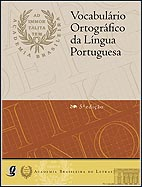
\includegraphics{imagens/capavolp.png}
	\label{fig:capavolp}
  \source{disponível em \url{http://www.academia.org.br/nossa-lingua/vocabulario-ortografico}..}
\end{figure}

Segundo a figura \ref{fig:capavolp}.
\subsubsection{Níveis de indentação}
Evite muitos níveis de indentação. Esse é o quarto nível (modelo Título 4). Embora possa haver outros níveis de indentação, 4 níveis é o máximo recomendado.
\subsection{Gramática e estilo}
Empregue sempre a gramática correta no seu texto. Estilo é uma forma individual de escrita. No gênero literário de escrita técnica, o estilo pode variar entre os autores, mas algum rigor deve ser seguido. Nos parágrafos seguintes serão apresentadas algumas dicas que, se seguidas, não serão criticados pela banca e farão seu texto ser mais atrativo para o leitor.

A seguir são apresentados alguns erros típicos de gramática que não devem ocorrer e algumas expressões ou termos que podem ser escritos por questões de estilo.

\begin{enumerate}[label=\alph*)]
\item {\bfseries Uso da abreviação “etc.”}

O termo “etc.” é a abreviação da expressão em latim “et cetera”, que significa “e outras coisas”. Como trata-se de uma abreviação, deve terminar com um ponto mesmo que esteja no meio da frase, seguindo-se por letra minúscula na palavra subsequente. Se terminar uma frase, basta o ponto de final de período. Como etc. já traz consigo o “e”, não deve ser escrito “e etc.”, nem tampouco deve ser precedido por vírgula. O uso de vírgula antes do etc. pode ser aceito na gramática moderna, mas a linguagem formal tradicional não a permite. Evite usar vírgula antes do etc. Nunca utilize reticências (“...”) após o etc.

\item {\bfseries Separar sujeito do predicado em uma oração}

O correto uso de vírgulas num texto técnico não é difícil, mas requer a atenção para algumas regras básicas. Um dos erros mais comuns é separar o sujeito do predicado por vírgulas, o que é um erro. Por exemplo:
“As pesquisas realizadas, indicaram que o resultado foi positivo.”
O sujeito desta frase é “as pesquisas realizadas” e o predicado é “indicaram que o resultado foi positivo”. Assim sendo, não pode ser utilizada vírgula para os separar.

\item {\bfseries Uso do advérbio “mesmo” como pronome}

Esse é um erro fatal que emporcalha o texto. Infelizmente, uma legislação municipal no Rio de Janeiro (e em alguns outros munícipios) propagou um erro de gramática, nos obrigando a ler: “Antes de entrar no elevador, verifique se o mesmo está parado neste andar”. Nesse caso, o termo “mesmo” traz o sentido de um pronome, que se trata de uma classe gramatical da qual o termo “mesmo” não faz parte. O correto seria escrever “Antes de entrar no elevador, verifique se ele está parado neste andar”.

Dica: sempre que for usar o termo “mesmo” ou “mesma”, verifique se pode ser substituído por “ele”, “ela” ou por outro pronome. Se a frase fizer sentido, então não use “mesmo” mas sim o pronome apropriado.
\item {\bfseries Iniciar frase com “E”}

A conjunção aditiva “e” não deve ser utilizado para iniciar. Conjunções são termos que ligam duas ou mais palavras ou orações das mesmas classes gramaticais. Assim sendo, não é gramaticalmente correto iniciar uma frase com conjunção aditiva.

\item {\bfseries Uso de “e/ou”}

Esse é um tema um tanto controverso. A norma culta da língua portuguesa prescinde do “e/ou” uma vez que o “ou” é não excludente. Isto é, “ou” é uma disjunção não exclusiva, portanto é equivalente ao “e/ou”. Na norma culta, a disjunção exclusiva é dada pelo “ou ... ou”. Por exemplo, para deixar a entender que um laboratório é exclusivamente de calibração ou exclusivamente de ensaio, a norma culta define que seria escrito assim: “... laboratório ou de ensaio ou de calibração”, ou alguma redação semelhante.

Entretanto, vale mencionar que hoje em dia se aceita o “e/ou” em linguagem cotidiana, portanto se trata de estilo usar ou não. Como sugestão, empregue o “e/ou” apenas em casos que a ausência do “e/” venha a trazer confusão no entendimento do texto. Repetindo: o “ou” na língua portuguesa tem o sentido de não exclusividade, portanto já contempla o sentido do “e/”.

\item {\bfseries Diferença entre ilustração e tabela}

Tabelas são elementos da estrutura de um texto técnico nas quais as principais informações transmitidas são números. Por outro lado, ilustrações podem ser desenhos, esquemas, fluxogramas, fotografias, gráficos, mapas, organogramas, plantas, quadros, retratos etc. Todos estes elementos podem ser genericamente denominados ilustrações, ou especificamente para cada tipo de ilustração. Cada tipo de elemento deve ser enumerado independentemente por ordem de aparecimento no texto. Embora não sejam elementos obrigatórios, geralmente são inseridas listas de tabelas e de ilustrações. A seguir serão apresentados exemplos de tabela, quadro e figura.




%Exemplo de Tabela
\begin{table}[!ht]
		\centering
		\Caption{Quantidade  de dias dos meses do primeiro semestre do ano.}		
		\IBGEtab{}{
		
		    %\resizebox{15cm}{!}{%
		    \begin{adjustbox}{width=0.7\textwidth,center}
			\begin{tabular}{ccccccc}
		    	\toprule
				JAN & FEV & MAR & ABR & MAI & JUN & JUL \\
				\midrule 
				31 & 28 (ou 29) & 31 & 30 & 31 & 30 & 31\\
				\bottomrule
			\end{tabular}
			\end{adjustbox}
		}{
		}
		\source{elaboração própria}
		\label{tab:exemplo-1}
\end{table}


\begin{table}[h]
\centering
\caption{Cotação do dólar turismo na primeira semana de abril de 2020.}
\label{tab:my-table}
\begin{adjustbox}{width=0.4\textwidth,center}
\begin{tabular}{@{}ccc@{}}
\toprule
          & \multicolumn{2}{c}{Cotação em real} \\ \cmidrule(l){2-3} 
Data      & Compra           & Venda            \\
01ABR2020 & 5,2399           & 5,2404           \\
02ABR2020 & 5,2645           & 5,2651           \\
03ABR2020 & 5,2991           & 5,2997           \\
04ABR2020 & --               & --               \\
05ABR2020 & --               & --               \\
06ABR2020 & 5,2465           & 5,2471           \\
07ABR2020 & 5,2211           & 5,2217           \\ \bottomrule
\end{tabular}
\end{adjustbox}
\source{\url{https://www4.bcb.gov.br} [acessado em 23ABR2020].}
\end{table}

    \begin{quadro}[h!]
        \caption{Nomes, símbolos e grandezas das unidades do Sistema Interamericano de Metrologia.}
        % coloque aqui o seu quadro
        \centering
		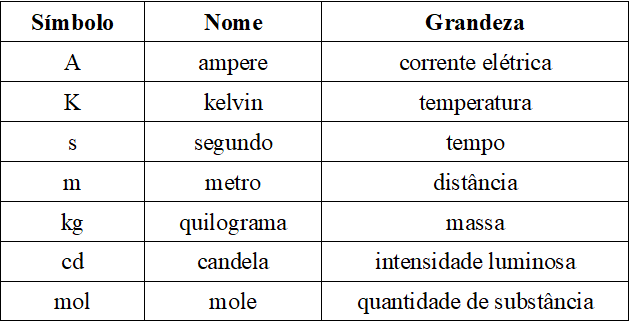
\includegraphics{imagens/Quadro grandezas.png}
	    \label{qd:grandezas}
	    \source{BIPM.}
    \end{quadro}
    
    %Exemplo de Figura
    
\begin{figure}[htbp]
    \caption{Exemplo de Figura.}
	\centering
		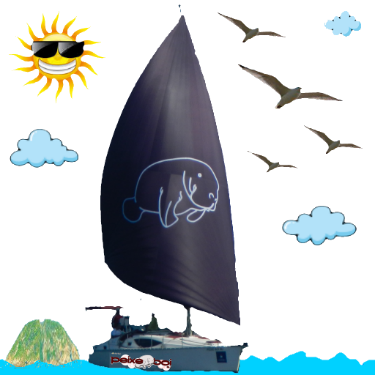
\includegraphics{imagens/barco.png}
	\source{elaboração própria.}
	\label{fig:barco}
\end{figure}

Observe que tanto tabelas quanto ilustrações (todos os tipos) devem ter a seguinte formatação: antes do elemento deve haver um título composto por “tipo” ou “palavra designativa” que pode ser desenho, esquema, fluxograma, fotografia, gráfico, mapa, organograma, planta, quadro, retrato, figura, imagem etc. A palavra designativa deve ser iniciada por letra maiúscula e demais letras minúsculas, seguida por um número de ordem de ocorrência no texto em algarismos arábicos, sucedido por um travessão ladeado por espaços simples (“ – ”) e seguido da descrição do elemento “título”, finalizando com um ponto simples. Após o elemento deve ser apresentada sua fonte mesmo que seja de elaboração própria. A grafia correta é, por exemplo: “Fonte: elaboração própria.”. “Fonte: adaptado de REFERÊNCIA.”; “Fonte: extraído de REFERÊNCIA.”. Observe que “Fonte” inicia-se por letra maiúscula e demais letras são minúsculas, seguindo-se dois pontos (“:”) e o texto a seguir deve ser iniciado por letras minúsculas, salvo nas classes gramaticais que demandar iniciarem-se por letras maiúsculas, como nomes próprios ou siglas, por exemplo. A apresentação da fonte deve ser finalizada por um ponto simples. As normas da ABNT são omissas quanto ao uso de ponto simples para finalizar a descrição do elemento (tabela ou ilustração). Entretanto, este guia faz uso desta formatação. O autor precisa ficar atento quando a fonte citar um site, pois o uso de ponto ao fina do site pode fazê-lo não ser identificado pelo navegador na internet. O tamanho da letra das descrições das tabelas, ilustrações e fontes é menor que a do corpo do texto. Neste guia, o tamanho do corpo do texto é 12 e destes elementos citados é 11 (ambos Times New Roman).

Quanto à formatação, a tabela não deve ter linhas verticais, a menos que sejam relevantes para melhor apresentar as informações. São obrigatórias três linhas horizontais em uma tabela: a que delimita o topo (ou início) da tabela; a que separa o topo do corpo (ou meio) da tabela; e a linha inferior que delimita o final da tabela. Outras linhas horizontais podem ser necessárias para melhor apresentação das informações, mas são dispensáveis. O documento que rege a elaboração de tabelas é o guia gerado pelo IBGE (IBGE, 1993).

\item {\bfseries Equações e fórmulas}
Todas as unidades devem ser baseadas na edição atual do Sistema Internacional de Unidades (SI). A seguir é apresentado um modelo para equações e fórmulas. As equações devem ser numeradas sequencialmente ao longo do texto e referenciadas no texto.

\begin{equation}
(x+a)^{n}=\sum_{k=0}^{n} 2^{-n}
\label{eqcargacap}
\end{equation}

\end{enumerate}


%
\section{Inserindo uma imagem}

Donec sit amet ex ante. Quisque porttitor velit diam, a maximus purus porta non. Sed vel massa pulvinar, tristique nulla id, convallis enim. Vestibulum hendrerit tempor faucibus. In lobortis eros felis, ac interdum velit tincidunt eget. Suspendisse posuere hendrerit purus, vitae blandit massa laoreet vitae. Donec iaculis consectetur erat, sed varius est pellentesque id. Donec at metus et nibh convallis ullamcorper. Maecenas rutrum scelerisque diam id accumsan. Phasellus non urna venenatis, efficitur urna nec, laoreet justo. Conforme \autoref{motor}:

%Exemplo de Figura
\begin{figure}[htbp]
    \caption{Bobby Icon - Um exemplo de como colocamos uma imagem...}
	\centering
		\includegraphics{imagens/bobby-icon.png}
	\legend{Fonte: Internet}
	\label{fig:image1}
\end{figure}

\begin{figure}[htbp]
    \caption{Exemplo de Motor}
	\centering
		\includegraphics[scale=0.5]{imagens/motor.jpeg}
	\legend{Fonte: Internet}
	\label{motor}
\end{figure}


Donec sit amet ex ante. Quisque porttitor velit diam, a maximus purus porta non. Sed vel massa pulvinar, tristique nulla id, convallis enim. Vestibulum hendrerit tempor faucibus. In lobortis eros felis, ac interdum velit tincidunt eget. Suspendisse posuere hendrerit purus, vitae blandit massa laoreet vitae. Donec iaculis consectetur erat, sed varius est pellentesque id. Donec at metus et nibh convallis ullamcorper. Maecenas rutrum scelerisque diam id accumsan. Phasellus non urna venenatis, efficitur urna nec, laoreet justo.

Lorem ipsum dolor sit amet, consectetur adipiscing elit. Quisque gravida sapien condimentum, tempor lectus vel, eleifend elit. Donec non aliquam elit. Nam at sapien sed felis fringilla aliquet ut quis mi. Sed pulvinar vulputate ante, et tincidunt tellus facilisis eget.

%Exemplo de Tabela
\begin{table}[!ht]	
		\centering
		\Caption{Exemplo de tabela}		
		\IBGEtab{}{
			\begin{tabular}{cll}
				\toprule
				Ranking & Exon Coverage & Splice Site Support \\
				\midrule \midrule
				E1 & Complete coverage by a single transcript & Both splice sites\\
				E2 & Complete coverage by more than a single transcript & Both splice sites\\
				E3 & Partial coverage & Both splice sites\\
				E4 & Partial coverage & One splice site\\
				E5 & Complete or partial coverage & No splice sites\\
				E6 & No coverage & No splice sites\\
				\bottomrule
			\end{tabular}
		}{
		\Fonte{Elaborado pelo autor}
		\label{tab:exemplo-1}
	}
\end{table}


\lipsum[24] Veja \autoref{tabela}:

\begin{table}[!ht]
\centering
\caption{Exemplo 2}
\label{tabela}
\begin{tabular}{ll}
\hline
\textbf{Ano} & \textbf{Quantidade} \\ \hline
2010         & 50                  \\ \hline
2012         & 200                 \\ \hline
2014         & 500                 \\ \hline
2016         & 300                 \\ \hline
\end{tabular}
\legend{Fonte: exemplo}
\end{table}

\section{Testes Finais}

Como disse \citeonline{LoremIpsum}: \lq\lq Lorem ipsum dolor sit amet, consectetur adipiscing elit. Quisque gravida sapien condimentum, tempor lectus vel, eleifend elit. Donec non aliquam elit. Nam at sapien sed felis fringilla aliquet ut quis mi. Sed pulvinar vulputate ante, et tincidunt tellus facilisis eget.\rq\rq

\begin{citacao}
Lorem ipsum dolor sit amet, consectetur adipiscing elit. Quisque gravida sapien condimentum, tempor lectus vel, eleifend elit. Donec non aliquam elit. Nam at sapien sed felis fringilla aliquet ut quis mi. Sed pulvinar vulputate ante, et tincidunt tellus facilisis eget.Lorem ipsum dolor sit amet, consectetur adipiscing elit. Quisque gravida sapien condimentum, tempor lectus vel, eleifend elit. Donec non aliquam elit. Nam at sapien sed felis fringilla aliquet ut quis mi. Sed pulvinar vulputate ante, et tincidunt tellus facilisis eget.
\end{citacao}

\lipsum[90-91]

%\include{capitulos/capitulo4}

%\include{capitulos/capitulo5}


% ----------------------------------------------------------
% ELEMENTOS PÓS-TEXTUAIS
% Se não tiver, pode apagar tudo até a penúltima linha
% ----------------------------------------------------------
\postextual

% ----------------------------------------------------------

% ----------------------------------------------------------
% Referências bibliográficas
% ----------------------------------------------------------

\bibliography{referencias}

% ----------------------------------------------------------
% Glossário
% ----------------------------------------------------------
% Consulte o manual da classe abntex2 para orientações sobre o glossário.
%\glossary


% Apêndices e anexos
% Segundo a NBR 14724 de dezembro de 2005, a diferença primordial entre Anexo e Apêndice é que o Anexo é um texto ou documento não elaborado pelo autor do Trabalho Científico (TC) (monografia, tese, etc.) e o Apêndice é um texto ou documento elaborado pelo autor do TC
% http://www.portalsaofrancisco.com.br/portugues/anexos-e-apendices
% Não é obrigatório

%\imprimirapendices %insere uma folha com o texto apendices para separar os apendices do restante do texto
\apendices
% Adicione aqui os apendices do seu trabalho
\apendice{Modelo de Capa} %título do apendice
\label{ap:modelo-de-capa}

\lipsum[1]
        
%\imprimiranexos %insere uma folha com o texto anexos para separar os anexos do restante do texto
\anexos
\anexo{Dinâmica das classes sociais}
\label{an:dinamica-das-classes-sociais}

\lipsum[14]
        
%---------------------------------------------------------------------
% INDICE REMISSIVO
%---------------------------------------------------------------------
% \phantompart
% \printindex
%---------------------------------------------------------------------

%Não apague essa linha
\end{document}